\documentclass[xetex,mathserif,serif]{beamer}
\usepackage{polyglossia}
\setdefaultlanguage[babelshorthands=true]{russian}
\usepackage{minted}

\useoutertheme{infolines}

\setmainfont{FreeSans}
\newfontfamily{\russianfonttt}{FreeSans}

\newcommand{\attribution}[1] {
    \begin{flushright}\begin{scriptsize}\textcolor{gray}{\textcopyright\, #1}\end{scriptsize}\end{flushright}
}

\title{Принципы объектно-ориентированного проектирования}
\author[Юрий Литвинов]{Юрий Литвинов \newline \textcolor{gray}{\small\texttt{yurii.litvinov@gmail.com}}}
\date{17.03.2021г}

\begin{document}
    
    \frame{\titlepage}

    \section{Объекты и классы}

    \begin{frame}
        \frametitle{Объекты}
        \begin{itemize}
            \item Objects may contain data, in the form of fields, often known as attributes; and code, in the form of procedures, often known as methods --- \textbf{\href{https://en.wikipedia.org/wiki/Object-oriented\_programming}{Wikipedia}}
            \item An object stores its state in fields and exposes its behavior through methods --- \textbf{\href{https://docs.oracle.com/javase/tutorial/java/concepts/object.html}{Oracle}}
            \item Each object looks quite a bit like a little computer --- it has a state, and it has operations that you can ask it to perform --- \textbf{\href{http://amzn.to/1PBmQpm}{Thinking in Java}}
            \item An object is some memory that holds a value of some type --- \textbf{\href{http://amzn.to/1XyGCtk}{The C++ Programming Language}}
            \item An object is the equivalent of the quanta from which the universe is constructed --- \textbf{\href{http://amzn.to/266oJr4}{Object Thinking}}
        \end{itemize}
    \end{frame}

    \begin{frame}
        \frametitle{Объекты}
        \begin{itemize}
            \item Имеют
            \begin{itemize}
                \item Состояние
                \begin{itemize}
                    \item Инвариант
                \end{itemize}
                \item Поведение
                \item Идентичность
            \end{itemize}
            \item Взаимодействуют через посылку и приём сообщений
            \begin{itemize}
                \item Объект вправе сам решить, как обработать вызов метода (\textbf{полиморфизм})
                \item Могут существовать в разных потоках
            \end{itemize}
            \item Как правило, являются экземплярами \textbf{классов}
        \end{itemize}
    \end{frame}

    \begin{frame}
        \frametitle{Абстракция}
        \textbf{Абстракция} выделяет существенные характеристики объекта, отличающие его от остальных объектов, с точки зрения наблюдателя
        \vskip 1cm
        \begin{center}
            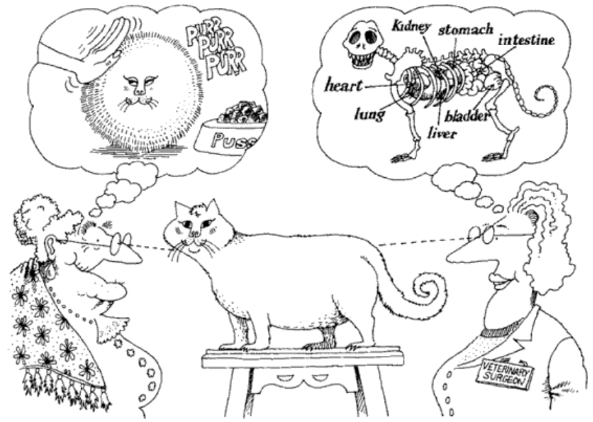
\includegraphics[width=0.45\textwidth]{abstraction.png}
        \end{center}
        \attribution{G. Booch, ``Object-oriented analysis and design''}
    \end{frame}

    \begin{frame}
        \frametitle{Инкапсуляция}
        \textbf{Инкапсуляция} разделяет абстракцию и её реализацию

        Инкапсуляция защищает \textbf{инварианты} абстракции
        \vskip 1cm
        \begin{center}
            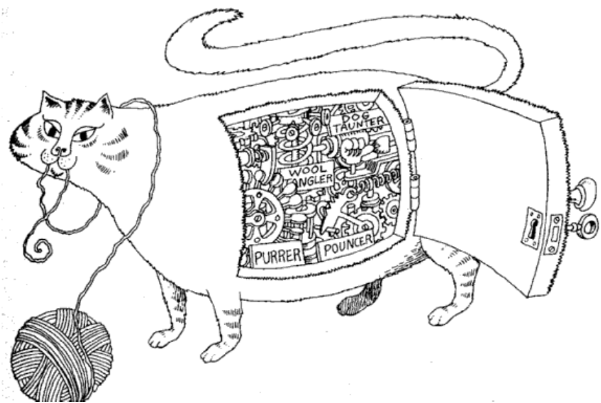
\includegraphics[width=0.45\textwidth]{incapsulation.png}
        \end{center}
        \attribution{G. Booch, ``Object-oriented analysis and design''}
    \end{frame}

    \begin{frame}
        \frametitle{Наследование и композиция}
        \begin{itemize}
            \item \textbf{Наследование}
            \begin{itemize}
                \item Отношение ``Является'' (is-a)
                \item Способ абстрагирования и классификации
                \item Средство обеспечения \textbf{полиморфизма}
            \end{itemize}
            \item \textbf{Композиция}
            \begin{itemize}
                \item Отношение ``Имеет'' (has-a)
                \item Способ создания динамических связей
                \item Средство обеспечения делегирования
            \end{itemize}
            \item Более-менее взаимозаменяемы
            \begin{itemize}
                \item Объект-потомок на самом деле включает в себя объект-предок
                \item Композиция обычно предпочтительнее
            \end{itemize}
        \end{itemize}
    \end{frame}

    \begin{frame}
        \frametitle{Откуда брать классы}
        \begin{itemize}
            \item Объектная модель предметной области
            \begin{itemize}
                \item Основной источник ``важных'' объектов
                \item Существительные --- классы, глаголы --- методы
            \end{itemize}
            \item Изоляция сложности
            \item Изоляция изменений
            \item Изоляция служебной функциональности
            \item Упаковка родственных операций
            \begin{itemize}
                \item Статические классы вполне ок
            \end{itemize}
        \end{itemize}
    \end{frame}

    \begin{frame}
        \frametitle{Предметно-ориентированное проектирование}
        \begin{itemize}
            \item Вся архитектура строится вокруг модели предметной области
            \item Модель как средство анализа и проектирования
            \item Единый язык
            \item Чёткое разделение на уровни
            \begin{itemize}
                \item Интерфейс пользователя
                \item Операционный
                \item Предметной области
                \item Инфраструктурный
            \end{itemize}
            \item Изоляция и минимизация модели предметной области
            \begin{itemize}
                \item Выделение смыслового ядра
            \end{itemize}
        \end{itemize}
    \end{frame}

    \section{Принципы SOLID}

    \begin{frame}
        \frametitle{Принципы SOLID}
        \begin{itemize}
            \item Single responsibility principle
            \item Open/closed principle
            \item Liskov substitution principle
            \item Interface segregation principle
            \item Dependency inversion principle
        \end{itemize}
    \end{frame}

    \begin{frame}
        \frametitle{Single responsibility principle}
        \begin{itemize}
            \item Каждый объект должен иметь одну обязанность
            \item Эта обязанность должна быть полностью инкапсулирована в класс
        \end{itemize}
        \begin{flushright}
            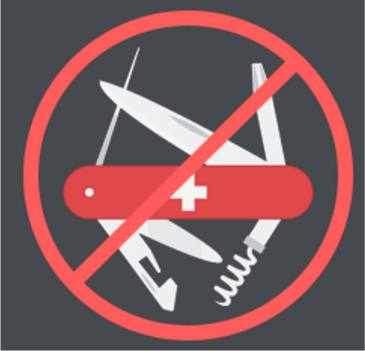
\includegraphics[width=0.25\textwidth]{singleResponsibility.png}
        \end{flushright}
    \end{frame}

    \begin{frame}
        \frametitle{Open/closed principle}
        \begin{itemize}
            \item программные сущности (классы, модули, функции и т. п.) должны быть открыты для расширения, но закрыты для изменения
            \begin{itemize}
                \item переиспользование через наследование
                \item неизменные интерфейсы
            \end{itemize}
        \end{itemize}
        \begin{flushright}
            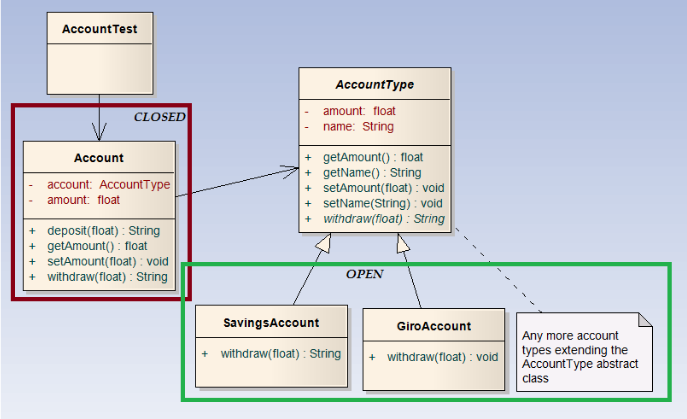
\includegraphics[width=0.5\textwidth]{openClosedPrinciple.png}
        \end{flushright}
    \end{frame}

    \begin{frame}
        \frametitle{Liskov substitution principle}
        \begin{itemize}
            \item Функции, которые используют базовый тип, должны иметь возможность использовать подтипы базового типа, не зная об этом
        \end{itemize}
        \begin{flushright}
            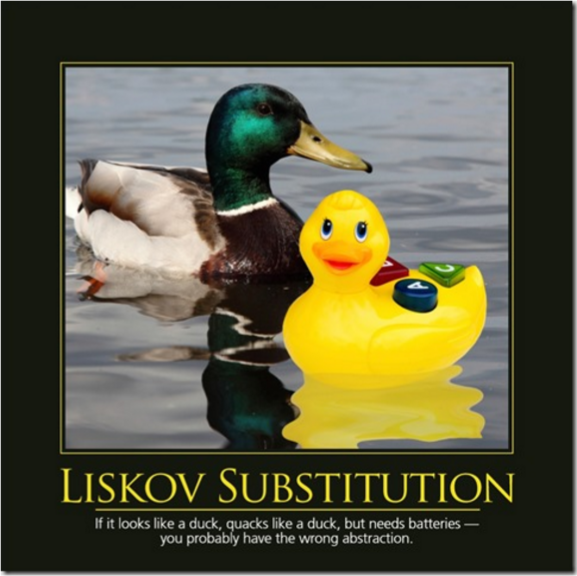
\includegraphics[width=0.4\textwidth]{liskovSubstitutionPrinciple.png}
        \end{flushright}
    \end{frame}

    \begin{frame}
        \frametitle{Interface segregation principle}
        \begin{itemize}
            \item Клиенты не должны зависеть от методов, которые они не используют
            \begin{itemize}
                \item слишком ``толстые'' интерфейсы необходимо разделять на более мелкие и специфические
            \end{itemize}
        \end{itemize}
        \begin{flushright}
            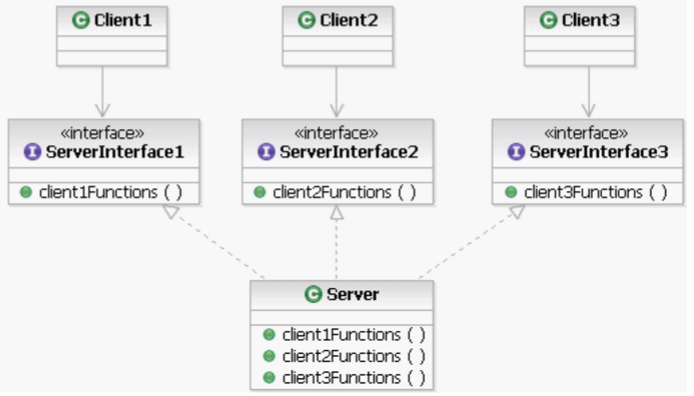
\includegraphics[width=0.5\textwidth]{interfaceSegregationPrinciple.png}
        \end{flushright}
    \end{frame}

    \begin{frame}
        \frametitle{Dependency inversion principle}
        \begin{itemize}
            \item Модули верхних уровней не должны зависеть от модулей нижних уровней. Оба типа модулей должны зависеть от абстракций
            \item Абстракции не должны зависеть от деталей. Детали должны зависеть от абстракций
        \end{itemize}
        \begin{flushright}
            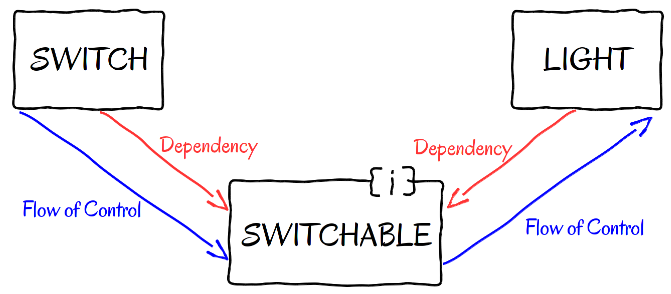
\includegraphics[width=0.5\textwidth]{dependencyInversionPrinciple.png}
        \end{flushright}
    \end{frame}

    \begin{frame}
        \frametitle{Закон Деметры}
        \begin{itemize}
            \item ``Не разговаривай с незнакомцами!''
            \item Объект A не должен иметь возможность получить непосредственный доступ к объекту C, если у объекта A есть доступ к объекту B, и у объекта B есть доступ к объекту C
            \begin{itemize}
                \item \mintinline{java}|book.pages.last.text|
                \item \mintinline{java}|book.pages().last().text()|
                \item \mintinline{java}|book.lastPageText()|
            \end{itemize}
        \end{itemize}
    \end{frame}

    \section{Абстракция}

    \begin{frame}[fragile]
        \frametitle{Пример плохой абстракции}
        \begin{minted}{java}
public class Program {
   public void initializeCommandStack() { ... }
   public void pushCommand(Command command) { ... }
   public Command popCommand() { ... }
   public void shutdownCommandStack() { ... }
   public void initializeReportFormatting() { ... }
   public void formatReport(Report report) { ... }
   public void printReport(Report report) { ... }
   public void initializeGlobalData() { ... }
   public void shutdownGlobalData() { ... }
}
        \end{minted}
\end{frame}

    \begin{frame}[fragile]
        \frametitle{Пример хорошей абстракции}
        \begin{footnotesize}
            \begin{minted}{java}
public class Employee {
   public Employee(
           FullName name,
           Address address,
           Phone workPhone,
           Phone homePhone,
           TaxId taxIdNumber,
   ) { ... }

   public FullName getName() { ... }
   public Address getAddress() { ... }
   public Phone getWorkPhone() { ... }
   public Phone getHomePhone() { ... }
   public TaxId getTaxIdNumber() { ... }
}
            \end{minted}
        \end{footnotesize}
\end{frame}

    \begin{frame}[fragile]
        \frametitle{Уровень абстракции (плохо)}
        \begin{minted}{java}
public class EmployeeRoster implements MyList<Employee> {
   public void addEmployee(Employee employee) { ... }
   public void removeEmployee(Employee employee) { ... }
   public Employee nextItemInList() { ... }
   public Employee firstItem() { ... }
   public Employee lastItem() { ... }
}
        \end{minted}
\end{frame}

    \begin{frame}[fragile]
        \frametitle{Уровень абстракции (хорошо)}
        \begin{minted}{java}
public class EmployeeRoster {
   public void addEmployee(Employee employee) { ... }
   public void removeEmployee(Employee employee) { ... }
   public Employee nextEmployee() { ... }
   public Employee firstEmployee() { ... }
   public Employee lastEmployee() { ... }
}
        \end{minted}
\end{frame}

    \begin{frame}
        \frametitle{Общие рекомендации}
        \begin{itemize}
            \item Про каждый класс знайте, реализацией какой абстракции он является
            \begin{itemize}
                \item Может потребоваться разделить класс на несколько разных классов просто потому, что методы по смыслу слабо связаны
            \end{itemize}
            \item Учитывайте противоположные методы (add/remove, on/off, ...)
            \item По возможности делайте некорректные состояния невыразимыми в системе типов
            \item \textit{Объясняющая способность программы важнее её работоспособности!}
        \end{itemize}
    \end{frame}

    \section{Инкапсуляция}

    \begin{frame}[fragile]
        \frametitle{Инкапсуляция}
        \begin{columns}
            \begin{column}{0.32\textwidth}
                \begin{minted}{java}
public class Point {
    public double x;
    public double y;
}
                \end{minted}
            \end{column}
            \begin{column}{0.05\textwidth}
                vs
            \end{column}
            \begin{column}{0.6\textwidth}
                \begin{minted}{java}
public interface Point {
    double getX();
    double getY();
    void setCartesian(double x, double y);
    double getR();
    double getTheta();
    void setPolar(double r, double theta);
}
                \end{minted}
            \end{column}
        \end{columns}
    \end{frame}

    \begin{frame}
        \frametitle{Ещё рекомендации}
        \begin{itemize}
            \item Класс не должен ничего знать о своих клиентах
            \item Опасайтесь семантических нарушений инкапсуляции
            \begin{itemize}
                \item ``Не будем вызывать ConnectToDB(), потому что GetRow() сам его вызовет, если соединение не установлено'' --- это программирование \textit{сквозь} интерфейс
            \end{itemize}
            \item Protected- и package- полей тоже не бывает
            \begin{itemize}
                \item На самом деле, у класса два интерфейса --- для внешних объектов и для потомков (может быть отдельно третий, для классов внутри пакета)
            \end{itemize}
        \end{itemize}
    \end{frame}

    \section{Наследование}

    \begin{frame}
        \frametitle{Наследование}
        \begin{itemize}
            \item Включение лучше
            \begin{itemize}
                \item Переконфигурируемо во время выполнения
                \item Более гибко
                \item Иногда более естественно
            \end{itemize}
            \item Наследование --- отношение ``является''
            \begin{itemize}
                \item Наследование --- это наследование интерфейса (полиморфизм подтипов, subtyping)
                \item Потомок принимает на себя обязательства предка
            \end{itemize}
            \item Code smells:
            \begin{itemize}
                \item Базовый класс, у которого только один потомок
                \item Пустые переопределения
                \item Очень много уровней в иерархии наследования
            \end{itemize}
        \end{itemize}
    \end{frame}

    \begin{frame}[fragile]
        \frametitle{Пример}
        \begin{footnotesize}
            \begin{columns}
                \begin{column}{0.35\textwidth}
                    \begin{minted}{java}
class Operation {
   private char sign = '+';
   private int left;
   private int right;
   public int eval()
   {
       switch (sign) {
           case '+': return left + right;
           ...
       }
       throw new RuntimeException();
   }
}
                    \end{minted}
                \end{column}
                \begin{column}{0.1\textwidth}
                    vs
                \end{column}
                \begin{column}{0.45\textwidth}
                    \begin{minted}{java}
abstract class Operation {
   private int left;
   private int right;
   protected int getLeft() { return left; }
   protected int getRight() { return right; }
   abstract public int eval();
}

class Plus extends Operation {
   @Override public int eval() { 
        return getLeft() + getRight(); 
   }
}
                    \end{minted}
                \end{column}
            \end{columns}
        \end{footnotesize}
    \end{frame}

    \section{Общие рекомендации}

    \begin{frame}
        \frametitle{Общие рекомендации}
        \begin{itemize}
            \item Fail Fast
            \begin{itemize}
                \item Не доверяйте параметрам, переданным извне
                \item assert-ы -- чем больше, тем лучше
            \end{itemize}
            \item Документируйте все открытые элементы API
            \begin{itemize}
                \item И заодно всё остальное, для тех, кто будет это сопровождать
                \item Предусловия и постусловия, исключения, потокобезопасность
            \end{itemize}
            \item Статические проверки и статический анализ лучше, чем проверки в рантайме
            \begin{itemize}
                \item Используйте систему типов по максимуму
            \end{itemize}
            \item Юнит-тесты
            \item Continious Integration
            \item Не надо бояться всё переписать
        \end{itemize}
    \end{frame}

    \begin{frame}
        \frametitle{Заключение}
        \begin{columns}
            \begin{column}{0.5\textwidth}
                \begin{center}
                    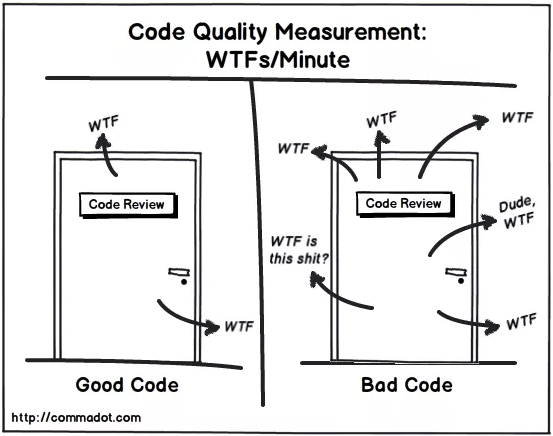
\includegraphics[width=0.7\textwidth]{wtfsMin.png}
                \end{center}
                \vspace{-0.8cm}
                \attribution{http://commadot.com, Thom Holwerda}
            \end{column}
            \begin{column}{0.5\textwidth}
                \begin{center}
                    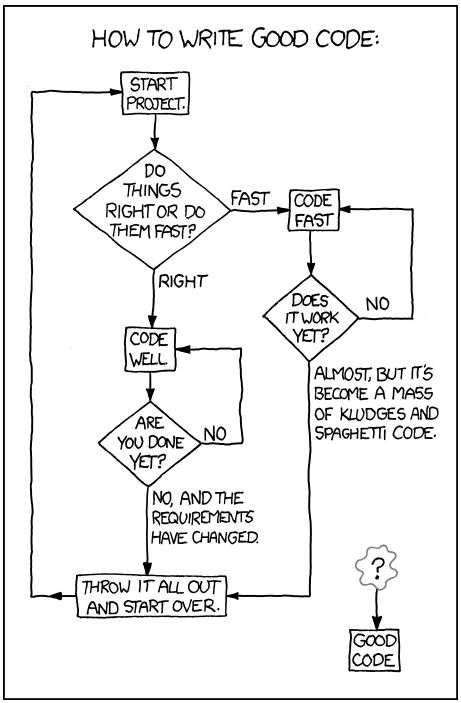
\includegraphics[width=0.7\textwidth]{goodCodeXkcd.png}
                \end{center}
                \vspace{-0.8cm}
                \attribution{https://xkcd.com}
            \end{column}
        \end{columns}
    \end{frame}

\end{document}